\chapter{Implementation}\label{chap:5}
In this chapter, the work of implementing malware classification system will be described. Starting with the implementing environment, this chapter will go through introduction of the meta-data used in
this system, and finally system software implementation which is written in PHP language.
%EXPERIMENTAL RESULTS AND ANALYSIS
%
%
\section{Environment}

In proposing system, operator system, Database, and are all operated in one computer. Technical information of employed computer is shown as in Table \ref{table:environment}. DecisionTree $1.5$ is good choice to this implementation, with these following reasons:
\begin{itemize}
\item The library constructs a decision tree from multidimensional training data.
\item The library use the decision tree thus constructed for classifying unlabeled data. \cite{decisiontreelibrary}.
\end{itemize} 
  \begin{table}
\begin{center}  
\label{table:environment}
    \begin{tabular}{ | l | l | l | }
     \hline
    Element &  Attribute  &  Environment \\ \hline
    OS & Computer & Ubuntu 11.04 \\ \hline
	Database & Mysql & Mysql 5.0 \\ \hline
	Programming language & C & gcc  \\ \hline
	 & PHP & PHP 5.0  \\ \hline
	 & Python & Python 2.7 \\ \hline
	 Library & DecisionTree 1.5 &  ID3 \\ \hline
    \end{tabular}
    \caption{Implementation environment of the malware classification system.}  
    \end{center}
  \end{table}
  
\section{Overview}
The system uses machine learning technique, named decision tree algorithm for malware classification. The goal is classifying malware fast and decision tree algorithm is used to achieve. Classification is a form of supervised learning, which requires training data, with known input/output, to form knowledge \cite{tonylee}. As mentioned in Figure \ref{fig:system_architec}, the system contains three following parts.

\begin{itemize}
\item First part: Read binary file to take meta data and input to database.
\item Second part: Manually cluster malware loaded from database.
\item Third part: Use decision tree algorithm to classify malware.
\end{itemize}
\begin{figure}[h!]
\centering
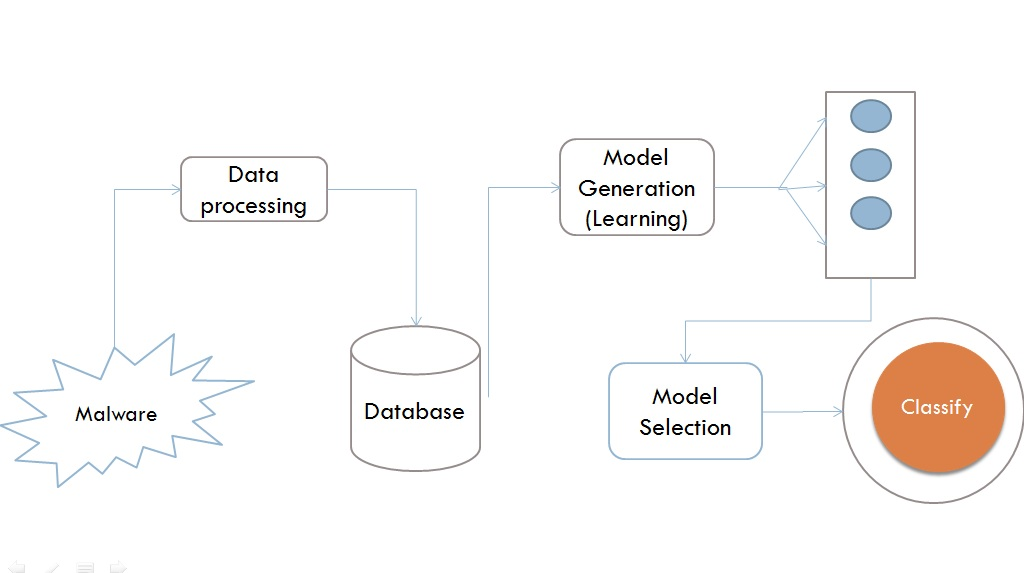
\includegraphics[width=1\textwidth]
{graph/system_architec.jpg}
\caption{The system architecture.}
\label{fig:system_architec}
\end{figure}

A vast amount of malware need analyzing, and the system uses database to store malware file's meta-data, to easily control a large number of data and to share them in the internet among web browsers.
The flow of data is shown in the Figure \ref{fig:system_architec}. At first, binary file meta-data are read, and all of the meta-data are input into database. In the second part, the system exports meta-data in database as the training data to create the decision tree for classifying malware. Finally, the decision tree algorithm created in the second step is utilized to class  unknown malware into the different malware families. 
%CLASSFICATION BASE ON DECISION TREE
%
%
\section{Classification based on machine learning technique} 
\subsection{Meta-data}
Meta-data is simply data about data. The malware file's meta-datas are all simply information about malware file. PE header includes meta-data of MS-DOS section; COFF file header; Optional header; Section header; and other types of data in sections include API import and export table. Meta-datas are many data about malware. The classification system based on can identify malware changed malware signature and syntax by using code reordering, code rewriting, and instruction insertion. Additionally, malware's meta-data can be easy received. 
Therefore, in order to create a fast and accuracy malware classification system, the system only uses PE header's meta-data to classify malware.
 
There is a problem that PE file's meta data value is too large to detect unknown malwares which have meta-data's differences from the training data of the system. The meta-data of PE header file are separated  to give semantic information for malware classification. For example, normally \emph{ImageBase} field of PE header file has value of 400000h \cite{goppit}. In this system, the meta-data of PE header file is separated into $7$ class by this calculation:
\begin{equation}
SemanticMetaData = MetaData \bmod 7
\end{equation} 

Decision tree modeling predicts effects $7$ is larger enough to separate malware file's meta-data value into classes. Additionally, $7$ is a prime number so that it is better to divide malware file's meta-data value into $7$ classes than another number. For example, The \emph{MajorLinkerVersion} field in PE file has a list of values as: $0x00003000$, $0x00001000$, and $0x00006000$. By the above equation, the semantic value of these value is as follows: 3,1,6. However, if the system use $8$, the semantic value of these value are as follows: 0. In conclusion, $7$ is good choice to separate malware file's meta-data value.

\subsection{Create training data}

In this system use decision tree technique. The attributes of decision tree described in previous subsection. Then, we mentions the method of identifying malware family name based on malware name provided by anti-virus vendors.

This research applies virustotal service to take the name of malware provided by the vendors and uses it to cluster malware into malware families with semantic information.

Figure \ref{fig:clustering} indicates HTTP post technique to automatically get name from virus total service and cluster malware into malware families which given in Figure \ref{fig:familymalware}.

Malware families in this classification system are as follows: Win32/Virut, Win32/Autorun, Win32/IRCbot, Win32/Gaobot, Win32/Waledac, Win32/Downadup, Win32/Sality, and W32.Mota. 

The disadvantage of using Virustotal to identify malware's families that a unique malware has many different names provided by many antis-virus vendors. Therefore, if unique malware has two or more families name provided by anti-virus vendor, unique malware will be classed into the most reported malware family.
\begin{figure}[h!]
\centering
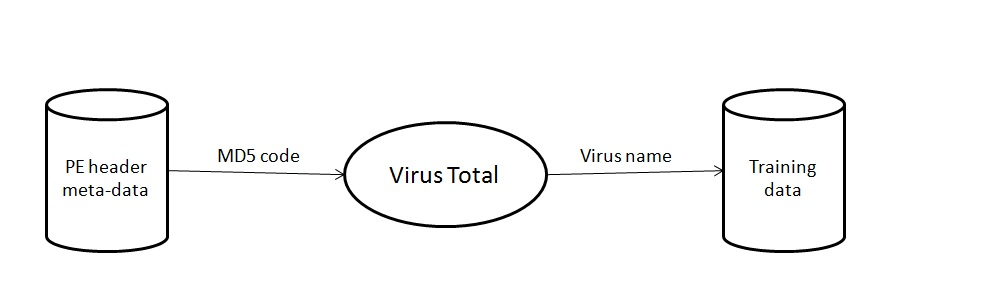
\includegraphics[width=1\textwidth]{graph/clustering.jpg}
\caption{Clustering method.}
\label{fig:clustering}
\end{figure}

\subsection{Classification}
\begin{figure}[h!]
\centering
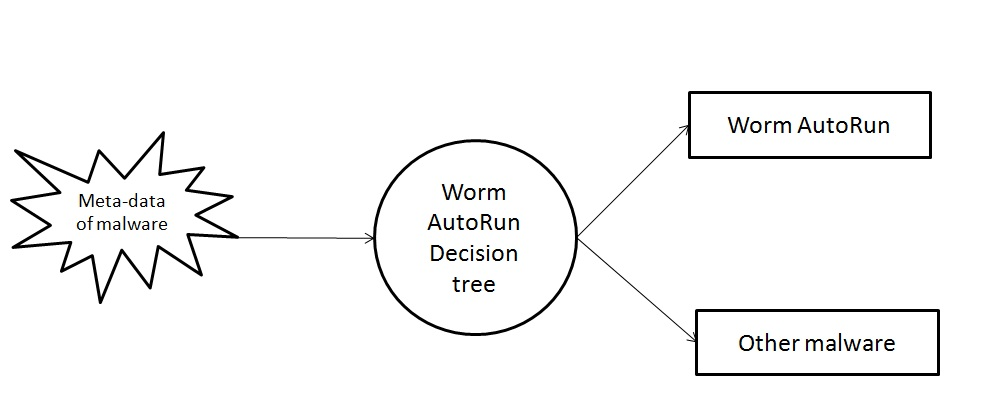
\includegraphics[width=1\textwidth]{graph/classificationdecision.jpg}
\caption{Worm autorun decision tree.}
\label{fig:classificationdecision}
\end{figure}

To make malware classification rapid and correct, decision tree algorithm is utilized. At that time, it is easy to update a new malware family, the classification uses decision tree algorithm to determine each malware family. For example, based on training data from clustering part, six decision trees are created. The worm autorun decision tree is indicated in Figure \ref{fig:classificationdecision}.

Malware' meta-data are known as input data for each decision tree, and the decision tree determines whether the malware is of worm autorun family or not. If the input malware belongs to worm autorun, malware classification shall detect which the family that malware is, otherwise it moves to the next decision tree. Lists of malware PE header file's meta-data are Magic, MajorLinkerVersion, MinorLinkerVersion, SizeOfCode, SizeOfInitializedData, SizeOfUninitializedData, AddressOfEntryPoint, BaseOfCode, BaseOfData, ImageBase, SectionAlignment, FileAlignment, MajorOperatingSystemVersion, MinorOperatingSystemVersion, MajorImageVersion, MinorImageVersion, MajorSubsystemVersion, MinorSubsystemVersion, Reserved1, SizeOfImage, SizeOfHeaders, CheckSum, Subsystem, DllCharacteristics, SizeOfStackReserve, SizeOfStackCommit, SizeOfHeapReserve, SizeOfHeapCommit, LoaderFlags, NumberOfRvaAndSizes, Machine, NumberOfSections, TimeDateStamp, PointerToSymbolTable, NumberOfSymbols, SizeOfOptionalHeader, Characteristics. The value of each field in PE header has semantics for decision tree algorithm if it is appeared at 10\% in malware training data. With this approach, the semantic value list of meta-data malware is made. For example, this is a list of meta-data created :1, 2, 6, 4, 0, 1, 1, 4, 0, 200, 4, 0, 0, 0, 4, 0, 0, 1.00E+00, 200, 0, 2, 0, 100000, 4000, 100000, 1000, 0, 10, 14c, 2, 1000, 8, 0, e0, 3, 818e. This is value before being computed :35328, 10b, 2, 0, 6200, 0, 200, b32e, b000, 9000, 400000, 1000, 200, 3, 0, 0, 0, 4, 0, 0, d000, 400, afe8, 2, 0, 1000, 1000, 10000, 0, 0, 10, 14c, 6, 0, 0, 0, e0, 10e. 
The malware classification part is shown in Figure \ref{fig:classification}. The training data from the malware clustering part is used to create the order of decision tree that makes malware classification system correct.
The decision tree is given as in Figure \ref{fig:decisiontreeworm}. When PE header's meta-data of malware is inputted into the worn autorun decision tree for determining unknown malware. Then, it decides whether it belongs to worm auto run family or not.
\begin{figure}[h!]
\centering
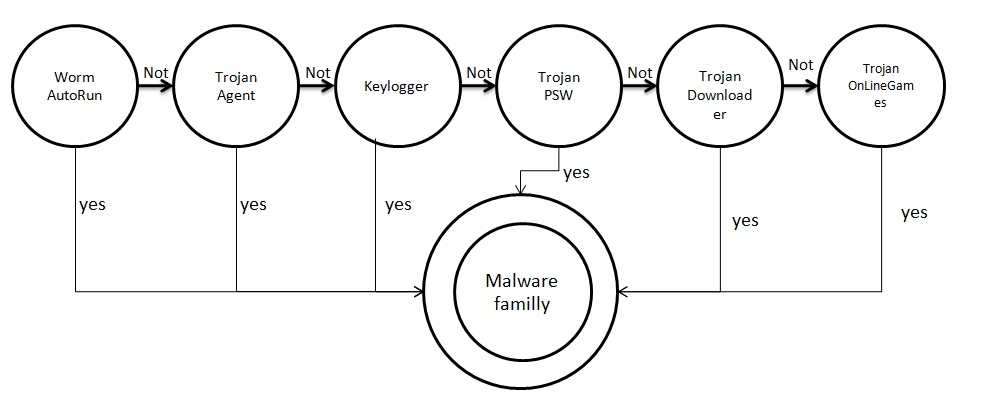
\includegraphics[width=1\textwidth]{graph/classification.jpg}
\caption{Malware classification system.}
\label{fig:classification}
\end{figure}
\begin{figure}[h!]
\centering
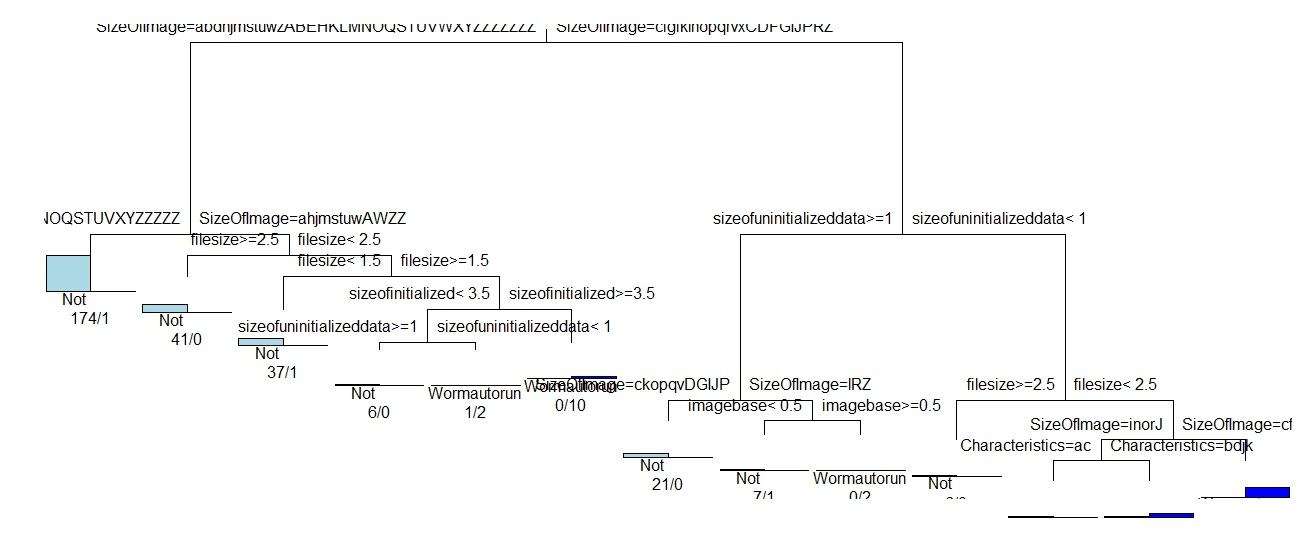
\includegraphics[width=1\textwidth]{graph/decisiontreeworm.jpg}
\caption{Worm autorun decision tree.}
\label{fig:decisiontreeworm}
\end{figure}
